\title{Deila og drottna}
\author{Bergur Snorrason}
\date{\today}

\begin{document}

\frame{\titlepage}

\env{frame}
{
    \frametitle{Almennar nálganir lausna}
    \env{itemize}
    {
        \item<1-> Þegar við leysum dæmi í keppnisforritun notumst við oftast við eina af eftirfarandi aðferðum:
        \env{itemize}
        {
            \item<2-> \emph{Ad hoc}.
            \item<3-> \emph{Tæmandi leit} eða \emph{ofbeldis aðferðin} (e. \emph{complete search, brute force}),
            \item<4-> \emph{Gráðug reiknirit} (e. \emph{greedy algorithms}),
            \item<5-> \emph{Deila og drottna} (e. \emph{divide and conquer}),
            \item<6-> \emph{Kvik bestun} (e. \emph{dynamic programming}).
        }
        \item<7-> Í síðustu vikum fjölluðum við um Ad hoc dæmi, tæmandi leit og gráðug reiknirit.
        \item<8-> Í þessari viku fjöllum við um deila og drottna reiknirit og kvika bestun.
    }
}

\env{frame}
{
    \frametitle{Deila og drottna}
    \env{itemize}
    {
        \item<1-> Sum dæmi má endurkvæmt skipta upp þangað til þau verða fáfengileg.
        \item<2-> Síðan má líma fáfengilegu lausnirnar saman í heildarlausn í lokinn.
        \item<3-> Slík reiknirit kallast \emph{deila og drottna} reiknirit.
        \item<4-> Þessi flokkur er sjaldgæfastur í keppnum.
        \item<5-> Það eru þó mörg þekkt reiknirit sem nýta sér deila og drottna.
    }
}

\env{frame}
{
    \frametitle{Deila og drottna, þekkt dæmi}
    \env{itemize}
    {
        \item<1-> Mergesort.
        \item<2-> Helmingunarleit (e. \emph{binary search}).
        \item<3-> Þriðjungaleit (e. \emph{ternary search}).
        \item<4-> Margföldunarreiknirit Karatsuba.
        \item<5-> Margföldunarreiknirit Strassen.
        \item<6-> Nálægustu punktar í plani.
        \item<7-> Fourier ummyndun (e. \emph{fast Fourier transform} (\ilcode{FFT})).
    }
}

\env{frame}
{
    \frametitle{Merge}
    \env{itemize}
    {
        \item<1-> Gerum ráð fyrir að við séum með tvo raðaða lista, $a$ og $b$.
        \item<2-> Búum til nýjan, tóman lista $c$.
        \item<3-> Berum saman fremstu stök $a$ og $b$ og tökum minna stakið og setjum aftast í $c$.
        \item<4-> Endurtökum þangað til $a$ eða $b$ er tómur.
        \item<5-> Skeytum svo því sem er eftir aftan á $c$.
        \item<6-> Nú inniheldur $c$ þau stök sem voru í $a$ og $b$ áður.
        \item<7-> Einnig er $c$ raðaður.
        \item<8-> Ef fjöldi staka í $a$ og $b$ er $n$ þá er þetta $\mathcal{O}($\onslide<9->{$\,n\,$}$)$.
    }
}

\defverbatim{\mergeA}
{ \begin{verbatim}
        a = [1, 2, 5, 6, 8, 9]
        b = [0, 3, 4, 7, 10]
        c = []
\end{verbatim} }

\defverbatim{\mergeB}
{ \begin{verbatim}
        a = [1, 2, 5, 6, 8, 9]
        b = [3, 4, 7, 10]
        c = [0]
\end{verbatim} }

\defverbatim{\mergeC}
{ \begin{verbatim}
        a = [2, 5, 6, 8, 9]
        b = [3, 4, 7, 10]
        c = [0, 1]
\end{verbatim} }

\defverbatim{\mergeD}
{ \begin{verbatim}
        a = [5, 6, 8, 9]
        b = [3, 4, 7, 10]
        c = [0, 1, 2]
\end{verbatim} }

\defverbatim{\mergeE}
{ \begin{verbatim}
        a = [5, 6, 8, 9]
        b = [4, 7, 10]
        c = [0, 1, 2, 3]
\end{verbatim} }

\defverbatim{\mergeF}
{ \begin{verbatim}
        a = [5, 6, 8, 9]
        b = [7, 10]
        c = [0, 1, 2, 3, 4]
\end{verbatim} }

\defverbatim{\mergeG}
{ \begin{verbatim}
        a = [6, 8, 9]
        b = [7, 10]
        c = [0, 1, 2, 3, 4, 5]
\end{verbatim} }

\defverbatim{\mergeH}
{ \begin{verbatim}
        a = [8, 9]
        b = [7, 10]
        c = [0, 1, 2, 3, 4, 5, 6]
\end{verbatim} }

\defverbatim{\mergeI}
{ \begin{verbatim}
        a = [8, 9]
        b = [10]
        c = [0, 1, 2, 3, 4, 5, 6, 7]
\end{verbatim} }

\defverbatim{\mergeJ}
{ \begin{verbatim}
        a = [9]
        b = [10]
        c = [0, 1, 2, 3, 4, 5, 6, 7, 8]
\end{verbatim} }

\defverbatim{\mergeK}
{ \begin{verbatim}
        a = []
        b = [10]
        c = [0, 1, 2, 3, 4, 5, 6, 7, 8, 9]
\end{verbatim} }

\defverbatim{\mergeL}
{ \begin{verbatim}
        a = []
        b = []
        c = [0, 1, 2, 3, 4, 5, 6, 7, 8, 9, 10]
\end{verbatim} }

\env{frame}
{
    \only<all:1> \mergeA
    \only<all:2> \mergeB
    \only<all:3> \mergeC
    \only<all:4> \mergeD
    \only<all:5> \mergeE
    \only<all:6> \mergeF
    \only<all:7> \mergeG
    \only<all:8> \mergeH
    \only<all:9> \mergeI
    \only<all:10> \mergeJ
    \only<all:11> \mergeK
    \only<all:12> \mergeL
}

\env{frame}
{
    \frametitle{Mergesort}
    \env{itemize}
    {
        \item<1-> Við getum notað þessa aðferð til að raða almennum lista.
        \item<2-> Við skiptum listanum okkar í tvo jafna hluta og köllum endurkvæmt á fallið okkar þangað til við erum með tómann lista.
        \item<3-> Á leiðinni upp úr endurkvæmninni sameinum við svo helmingana eins og rætt var á undan.
    }
}

\env{frame}
{
    \selectcode{code/mergesort.c}{6}{20}
}

\env{frame}
{
    \frametitle{Mergesort}
    \env{itemize}
    {
        \item<1-> Mergesort er sígilt dæmi um deila og drottna reiknirit.
        \item<2-> Við helmingum alltaf listann og tökum svo saman í línulegum tíma.
        \item<3-> Hvert stak kemur fyrir í $\mathcal{O}(\log n)$ sameiningum, svo reikniritið er $\mathcal{O}($\onslide<4->{$n \log n$}$)$.
        \item<5-> Þetta er mjög algeng tímaflækja í deila og drottna reikniritum.
    }
}

\env{frame}
{
    \frametitle{Helmingunarleit}
    \env{itemize}
    {
        \item<1-> Helmingunarleit er yfirleitt sett fram sem leit í röðuðum lista.
        \item<2-> Skoðum það fyrst og alhæfum svo.
        \item<3-> Látum $a$ vera raðaðan lista af $n$ tölum.
        \item<4-> Gerum ráð fyrir að við viljum finna $t$ í listanum.
        \item<5-> Látum $m = \lfloor n/2 \rfloor$.
        \item<6-> Ef $m$-ta stakið í $a$ er stærra en $t$ þá getur $t$ ekki verið í seinni helming listans.
        \item<7-> Ef $m$-ta stakið í $a$ er minna en $t$ þá getur $t$ ekki verið í fyrri helming listans.
        \item<8-> Svo við getum útilokað helming listans í hverri ítrun.
    }
}

\env{frame}
{
    \selectcode{code/bs-rec.c}{3}{9}
}

\env{frame}
{
    \env{itemize}
    {
        \item<1-> Helmingunarleit er $\mathcal{O}($\onslide<2->{$\log n$}$)$, þar sem við helmingum stærð listans í hverri ítrun.
        \item<3-> Góð æfing í helmingunarleit er að útfæra leitina þannig að hún skili vísi á fyrstu (eða síðustu)  endurtekningu staksins.
        \item<4-> Slíkar útgáfur að helmingunarleit nýtast þegar við förum að nota helmingunarleit í almennari mynd.
    }
}

\env{frame}
{
    \env{itemize}
    {
        \item<1-> Gerum ráð fyrir að við séum með vaxandi fall $f \colon [a, b] \rightarrow \mathbb{R}$ og $y \in \mathbb{R}$.
        \item<2-> Getum við fundið $x \in [a, b]$ þannig að $f(x) = y$?
        \item<3-> Slíkt $x$ þarf ekki að vera til, en ef $f$ er samfellt og $y \in [f(a), f(b)]$ þá er það til.
        \item<4-> En hvernig finnum við slíkt $x$?
        \item<5-> Við getum notað nákvæmlega sömu hugmynd og í helmingunarleit í lista.
        \item<6-> Látum $m = (a + b)/2$.
        \item<7-> Ef $f(m) > t$ þá þarf $x \in [a, m]$.
        \item<8-> Ef $f(m) < t$ þá þarf $x \in [m, b]$.
    }
}

\env{frame}
{
    \frametitle{Sýnidæmi}
    \env{center}
    {
        \env{tikzpicture}
        {
            [domain = -0.2:4.2]
            \draw[->] (-0.2,0) -- (4.2,0);
            \draw[->] (0,-0.2) -- (0,4.2);
            \draw[color=red] plot[id=c] function{2} node[right] {$y$};
            \draw[color=blue] plot[id=poly3] function{0.9 + 1.08333*x - 0.75*x**2 + 0.166667*x**3} node[right] {$f(x)$};



            \node<all:1-2>[below] at (0.7,-0.125) {$a$};
            \draw<all:1-2> (0.7,0.125) -- (0.7,-0.125);
            \draw<all:1-2>[dashed, gray] (0.7,0.125) -- (0.7, 4.2);
            \node<all:1-6>[below] at (3.7,-0.125) {$b$};
            \draw<all:1-6>(3.7,0.125) -- (3.7,-0.125);
            \draw<all:1-6>[dashed, gray] (3.7,0.125) -- (3.7,4.2);

            \node<all:2>[below] at (2.2,-0.125) {$m$};
            \draw<all:2-4> (2.2,0.125) -- (2.2,-0.125);
            \draw<all:2-4>[dashed, gray] (2.2,0.125) -- (2.2,4.2);

            \node<all:3-4>[below] at (2.2,-0.125) {$a$};

            \node<all:4>[below] at (2.95,-0.125) {$m$};
            \draw<all:4-> (2.95,0.125) -- (2.95,-0.125);
            \draw<all:4->[dashed, gray] (2.95,0.125) -- (2.95,4.2);

            \node<all:5->[below] at (2.95,-0.125) {$a$};

            \node<all:6>[below] at (3.325,-0.125) {$m$};
            \draw<all:6-> (3.325,0.125) -- (3.325,-0.125);
            \draw<all:6->[dashed, gray] (3.325,0.125) -- (3.325,4.2);

            \node<all:7->[below] at (3.325,-0.125) {$b$};
        }
    }
}

\env{frame}
{
    \env{itemize}
    {
        \item<1-> Takið eftir við munum ekki beint finna $x \in [a, b]$ þannig að $f(x) = y$.
        \item<2-> Það sem við finnum er $x \in [a, b]$ þannig að $|f(x) - y| < \varepsilon$, fyrir hvaða $\varepsilon > 0$ sem vera skal.
        \item<3-> Það er þó aldrei ætlast til annars í keppnisforritun og skekkjan er alltaf gefin í úttakslýsingu dæma.
    }
}

\env{frame}
{
    \env{itemize}
    {
        \item<1-> Við getum alhæft frekar.
        \item<2-> Tökum dæmi.
        \item<3-> Þú átt $k$ ketti og $n$ bæli fyrir kettina þína, með $2 \leq k \leq n$.
        \item<4-> Öll bælin eru staðsett á gangi í íbúðinni þinni.
        \item<5-> Ganginum má lýsa sem talnalínu og staðsetningar kattabælanna eru þá tölurnar 
                    $0 < x_1 < x_2 < ... < x_n < 10^9$ á talnalínunni.
        \item<6-> En kettir eru einfarar svo þeir vilja hafa sem mesta fjarlægð í næsta kött.
        \item<7-> Þú átt að raða köttum á bælin þannig að nálægustu kettirnir eru sem lengst frá hvorum öðrum.
    }
}

\env{frame}
{
    \env{itemize}
    {
        \item<1-> Þetta dæmi má leysa með helmingunarleit.
        \item<2-> Byrjum á að svara annari spurningu:
        \env{itemize}
        {
            \item<3-> Er hægt að raða köttunum þannig að nálægustu kettirnir séu að minnsta kosti með fjarlægð $r$?
        }
        \item<4-> Þetta dæmi má leysa gráðugt.
        \item<5-> Við töpum aldrei á því að setja kött á bælið staðsett á $x_1$.
        \item<6-> Við megum þá ekki setja kött á bæli sem liggja í $[x_1, x_1 + r]$.
        \item<7-> Útilokum þau og veljum minnsta bælið sem er eftir, og endurtökum.
        \item<8-> Ef við komum fyrir $k$, eða fleiri, köttum svona þá er svarið við nýju spurningunni ``já'', en annars ``nei''.
        \item<9-> Þetta tekur $\mathcal{O}($\onslide<10->{$n$}$)$.
    }
}

\env{frame}
{
    \env{itemize}
    {
        \item<1-> Tökum þó eftir að ef við komum fyrir öllum köttunum með fjarlægð $r_0$ þá gerum við það líka fyrir $r < r_0$.
        \item<2-> Skilgreinum fall
        \[
            f(r) = \left \{ \begin{array}{l l}
            1, & \text{ef koma má fyrir $k$,}\\
              & \text{eða fleiri, köttum með fjarlægð $r$}\\
            0, & \text{annars}.
            \end{array}
            \right .
        \]
        \item<3-> Við getum nú umorðað upprunarlega dæmið sem: ``Finnið stærsta $r$ þannig að $f(r) = 1$''.
        \item<4-> En nú er fallið $f$ minnkandi (samkvæmt efsta punktinum á glærunni), svo við getum fundið slíkt gildi með helmingunar leit.
    }
}

\env{frame}
{
    \frametitle{Sýnidæmi}
    \env{center}
    {
        \env{tikzpicture}
        {
            \draw[->] (-0.2,0) -- (4.2,0);
            \draw[->] (0,-0.2) -- (0,2.2);
            \draw[color=blue] (0,1) -- (3.1,1);
            \draw[color=blue] (3.1,0) -- (4,0);
            \node[above] at (1.5,1) {$f(r)$};



            \node<all:1-2>[below] at (0.7,-0.125) {$a$};
            \draw<all:1-2> (0.7,0.125) -- (0.7,-0.125);
            \draw<all:1-2>[dashed, gray] (0.7,0.125) -- (0.7, 2.2);
            \node<all:1-6>[below] at (3.7,-0.125) {$b$};
            \draw<all:1-6>(3.7,0.125) -- (3.7,-0.125);
            \draw<all:1-6>[dashed, gray] (3.7,0.125) -- (3.7,2.2);

            \node<all:2>[below] at (2.2,-0.125) {$m$};
            \draw<all:2-4> (2.2,0.125) -- (2.2,-0.125);
            \draw<all:2-4>[dashed, gray] (2.2,0.125) -- (2.2,2.2);

            \node<all:3-4>[below] at (2.2,-0.125) {$a$};

            \node<all:4>[below] at (2.95,-0.125) {$m$};
            \draw<all:4-> (2.95,0.125) -- (2.95,-0.125);
            \draw<all:4->[dashed, gray] (2.95,0.125) -- (2.95,2.2);

            \node<all:5->[below] at (2.95,-0.125) {$a$};

            \node<all:6>[below] at (3.325,-0.125) {$m$};
            \draw<all:6-> (3.325,0.125) -- (3.325,-0.125);
            \draw<all:6->[dashed, gray] (3.325,0.125) -- (3.325,2.2);

            \node<all:7->[below] at (3.325,-0.125) {$b$};
        }
    }
}

\env{frame}
{
    \env{itemize}
    {
        \item<1-> Ef við látum $M = 10^9/\varepsilon$, þar sem $\varepsilon$ er leyfileg skekkja í dæminu, þá er lausnin
            $\mathcal{O}($\onslide<2->{$n \log M$}$)$.
        \item<3-> Hér gerum við ekki ráð fyrir að svarið sé heiltala.
        \item<4-> Ef við gerum ráð fyrir því verður tímaflækjan eins, nema með $M = 10^9$.
    }
}

\env{frame}
{
    \env{itemize}
    {
        \item<1-> Það sem við gerðum í raun var að breyta dæminu úr ``finnið minnsta/stærsta gildið þannig að...''
                    yfir í ``tökum ákveðið gildi og athugum hvort að...''.
        \item<2-> Þetta er algengasta notkunin á helmingunarleit í keppnisforritun.
        \item<3-> Algengt er að helmingunarleit af þessum toga sé hluti af erfiðum dæmum.
    }
}

\env{frame}
{
    \selectcode{code/kisur.c}{3}{25}
}

\env{frame}
{
    \env{itemize}
    {
        \frametitle{Þriðjungaleit}
        \item<1-> Gerum ráð fyrir að við séum með kúpt fall $f \colon [a, b] \rightarrow \mathbb{R}$.
        \item<2-> Munið að fall er kúpt ef $f(tx_1 + (1 - t)x_2) \leq tf(x_1) + (1 - t)f(x_2)$, fyrir öll $t \in [0, 1]$ og $x_1, x_2 \in [a, b]$.
        \item<3-> Hvernig finnum við útgildi (há- og lággildi) fallsins?
        \item<4-> Auðvelt er að finna hágildi.
        \item<5-> Gerum ráð fyrir að $f(a) \leq f(b)$.
        \item<6-> Fyrir öll $x \in [a, b]$ gildir þá að
        \[
            f(x) = f(at + (1 - t)b) \leq tf(a) + (1 - t)f(b)
        \]
        \[
            \leq tf(b) + (1 - t)f(b) = f(b),
        \]
        með $t = (x - b)/(a - b)$.
        \item<7-> Svo hágildi fæst í endapuntkunum $a$ eða $b$.
    }
}

\env{frame}
{
    \env{itemize}
    {
        \frametitle{Þriðjungaleit}
        \item<1-> Við getum fundið lággildið tölulega, svipað og með helmingunarleit.
        \item<2-> Við veljum punkta $m_1, m_2 \in [a, b]$ þannig að bilin $[a, m_1]$, $[m_1, m_2]$ og $[m_2, b]$ séu jafn löng.
        \item<3-> Við skoðum svo fallgildin $f(m_1)$ og $f(m_2)$.
        \item<4-> Ef $f(m_1) < f(m_2)$ þá getur lággildið ekki legið á bilinu $[m_2, b]$, svo við getum útilokað það bil í leitinni.
        \item<5-> Ef $f(m_2) < f(m_1)$ þá getur lággildið ekki legið á bilinu $[a, m_1]$, svo við getum útilokað það bil í leitinni.
        \item<6-> Ef $f(m_2) = f(m_1)$ þá þarf lággildið að liggja á bilinu $[m_1, m_2]$.
        \item<7-> Þetta stafar allt af því að kúpt föll taka hágildi í öðru hvorum endapunkta sinna.
    }
}

\env{frame}
{
    \env{center}
    {
        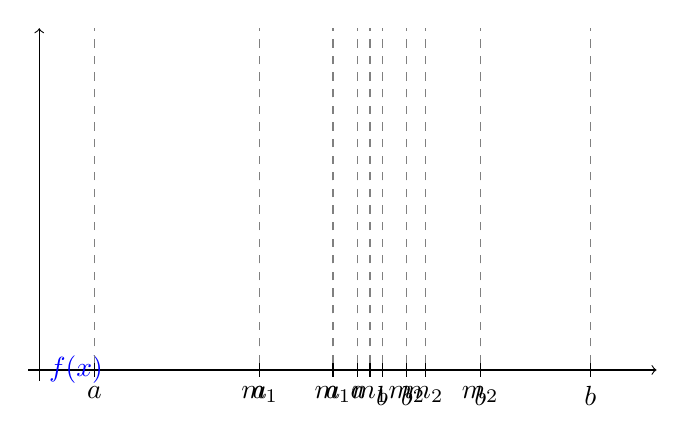
\begin{tikzpicture}[scale = 0.7, domain=-0.2:11.2]
            \draw[->] (-0.2,0) -- (11.2,0);
            \draw[->] (0,-0.2) -- (0,6.2);
            \draw[color = blue] plot[id=poly2] function{5 - 1.2*x + 0.1*x**2} node[right] {$f(x)$};

            \node<all:1-2>[below] at (1,-0.125) {$a$};
            \draw<all:1-2> (1,0.125) -- (1,-0.125);
            \draw<all:1-2>[dashed, gray] (1,0.125) -- (1, 6.2);

            \node<all:1-4>[below] at (10,-0.125) {$b$};
            \draw<all:1-4>(10,0.125) -- (10,-0.125);
            \draw<all:1-4>[dashed, gray] (10,0.125) -- (10,6.2);

            \node<all:2>[below] at (4,-0.125) {$m_1$};
            \draw<all:2>(4,0.125) -- (4,-0.125);
            \draw<all:2>[dashed, gray] (4,0.125) -- (4,6.2);

            \node<all:2>[below] at (7,-0.125) {$m_2$};
            \draw<all:2>(7,0.125) -- (7,-0.125);
            \draw<all:2>[dashed, gray] (7,0.125) -- (7,6.2);

            \node<all:3-6>[below] at (4,-0.125) {$a$};
            \draw<all:3-6> (4,0.125) -- (4,-0.125);
            \draw<all:3-6>[dashed, gray] (4,0.125) -- (4, 6.2);

            \node<all:4>[below] at (6,-0.125) {$m_1$};
            \draw<all:4>(6,0.125) -- (6,-0.125);
            \draw<all:4>[dashed, gray] (6,0.125) -- (6,6.2);

            \node<all:4>[below] at (8,-0.125) {$m_2$};
            \draw<all:4>(8,0.125) -- (8,-0.125);
            \draw<all:4>[dashed, gray] (8,0.125) -- (8,6.2);

            \node<all:5-6>[below] at (8,-0.125) {$b$};
            \draw<all:5-6>(8,0.125) -- (8,-0.125);
            \draw<all:5-6>[dashed, gray] (8,0.125) -- (8,6.2);

            \node<all:6>[below] at (5.33,-0.125) {$m_1$};
            \draw<all:6>(5.33,0.125) -- (5.33,-0.125);
            \draw<all:6>[dashed, gray] (5.33,0.125) -- (5.33,6.2);

            \node<all:6>[below] at (6.67,-0.125) {$m_2$};
            \draw<all:6>(6.67,0.125) -- (6.67,-0.125);
            \draw<all:6>[dashed, gray] (6.67,0.125) -- (6.67,6.2);

            \node<all:7-8>[below] at (5.33,-0.125) {$a$};
            \draw<all:7-8>(5.33,0.125) -- (5.33,-0.125);
            \draw<all:7-8>[dashed, gray] (5.33,0.125) -- (5.33,6.2);

            \node<all:7-8>[below] at (6.67,-0.125) {$b$};
            \draw<all:7-8>(6.67,0.125) -- (6.67,-0.125);
            \draw<all:7-8>[dashed, gray] (6.67,0.125) -- (6.67,6.2);

            \draw<all:8>(5.78,0.125) -- (5.78,-0.125);
            \draw<all:8>[dashed, gray] (5.78,0.125) -- (5.78,6.2);

            \draw<all:8>(6.22,0.125) -- (6.22,-0.125);
            \draw<all:8>[dashed, gray] (6.22,0.125) -- (6.22,6.2);

            \node<all:9>[below] at (5.78,-0.125) {$a$};
            \draw<all:9>(5.78,0.125) -- (5.78,-0.125);
            \draw<all:9>[dashed, gray] (5.78,0.125) -- (5.78,6.2);

            \node<all:9>[below] at (6.22,-0.125) {$b$};
            \draw<all:9>(6.22,0.125) -- (6.22,-0.125);
            \draw<all:9>[dashed, gray] (6.22,0.125) -- (6.22,6.2);
        \end{tikzpicture}
    }
}

\env{frame}
{
    \env{itemize}
    {
        \item<1-> Við notum okkur oft að tvídiffranlegt fall er kúpt ef og aðeins ef önnur afleiðan er jákvæð.
        \item<2-> Umfjöllunin okkar heimfærist á eðlilegan hátt yfir á hvelf föll.
        \item<3-> Þriðjungaleit er algeng í rúmfræði því Evklíðska firðin er kúpt.
    }
}

\env{frame}
{
    \selectcode{code/ts.c}{3}{21}
}

\env{frame}
{
    \env{itemize}
    {
        \item<1-> Tökum eitt hefðbundið sýnidæmi í lokinn.
        \item<2-> Þú vilt skortselja gjaldmiðil, vitandi framtíðargengi, þannig að þú græðir sem mestan pening.
        \item<3-> Nánar, þú ætlar að fá lánaðar $100$ danskar krónur á einhverjum degi og skipta þeim um leið í íslenskar krónur.
        \item<4-> Eftir einhvern fjölda daga þarft þú svo að kaupa $100$ danskar krónur til að borga lánið,
                    ásamt því að borga $K$ íslenskar krónur á dag í lánakostnað.
        \item<5-> Hver er mesti fjöldi íslenska króna sem þú getur grætt?
        \item<6-> Fyrsta lína inntaksins inniheldur tvær tölur, $1 \leq n \leq 10^5$ og $1 \leq k \leq 100$.
        \item<7-> Næsta lína inniheldur $n$ heiltölur $1 \leq x_1, x_2, ..., x_n \leq 10^5$.
        \item<8-> Hér tákna $x_i$ fjölda íslenska króna sem ein dönsk króna kostar á $i$-ta degi.
    }
}

\env{frame}
{
    \env{itemize}
    {
        \item<1-> Skoðum sýniinntök.
        \item<2->[]
        \code{code/shortsell.in}
        \item<3-> Í fyrra tilfellinu viljum við taka lánið á fyrsta degi og borga það á síðasta degi.
        \item<4-> Við fáum $100 \cdot 1000 = 10^5$ íslenskar krónur á fyrst degi og borgum $100 \cdot 10 = 10^3$ íslenskar krónur á síðasta degi.
        \item<5-> Við borgum svo $5 \cdot 10 = 50$ íslenskar krónur í lánakostnað.
        \item<6-> Svo við endum með $10^5 - 10^3 - 50 = 98950$ íslenskar krónur.
    }
}

\env{frame}
{
    \env{itemize}
    {
        \item<1-> Skoðum sýniinntök.
        \item<1->[]
        \code{code/shortsell.in}
        \item<1-> Í seinna tilfellinu viljum við taka lánið á fjórða degi og borga það á síðasta degi.
        \item<2-> Við fáum $100 \cdot 103 = 10300$ íslenskar krónur á fyrst degi og borgum $100 \cdot 100 = 10^4$ íslenskar krónur á síðasta degi.
        \item<3-> Við borgum svo $2 \cdot 100 = 200$ íslenskar krónur í lánakostnað.
        \item<4-> Svo við endum með $10300 - 10^4 - 200 = 100$ íslenskar krónur.
    }
}

\env{frame}
{
    \env{itemize}
    {
        \item<1-> Til að nota deila og drottna þurfum við að taka eftir einu.
        \item<2-> Gerum ráð fyrir að engin lánakostnaður sé greiddur síðasta daginn.
        \item<3-> Það einfaldar reikninga og við getum alltaf bætt honum við eftir á.
        \item<4-> Táknum með $f(i, j)$ þann gróða (eða tap) sem fæst með því að taka lánið á $i$-ta degi og borga það á $j$-degi degi,
                    og $g(i)$ vera gengið á $i$-ta degi.
        \item<5-> Við fáum nú að $f(i, j) = 100 \cdot g(i) - 100 \cdot g(j) - (j - i) \cdot k$.
        \item<6-> Ef $a$, $b$ og $c$ eru heiltölur þannig að $1 \leq a < b < c \leq n$ þá fæst
        \env{align*}
        {
            f(a, b) + f(b, c) =& 100 \cdot (g(a) - g(b)) - (b - a) \cdot k\\
                               &+ 100 \cdot (g(b) - g(c)) - (c - b) \cdot k\\
                              =& 100 \cdot (g(a) - g(c)) - (c - a) \cdot k\\
                              =& f(a, c).
        }
    }
}

\env{frame}
{
    \env{itemize}
    {
        \item<1-> Látum nú $m = \lfloor n/2 \rfloor$.
        \item<2-> Þá gildir eitt af þrennu, fyrir tiltekna lausn:
        \env{itemize}
        {
            \item<3-> Báðir endapunktar bestu lausnarinnar liggja á $[1, m - 1]$.
            \item<4-> Báðir endapunktar bestu lausnarinnar liggja á $[m, n]$.
            \item<5-> Annar endapunktur bestu lausnarinnar liggur á $[1, m - 1]$ og hinn liggur á $[m, n]$.
        }
        \item<6-> Fyrri tvö tilfellin má leysa með einfaldri endurkvæmni.
        \item<7-> Fyrir síðasta tilfellið nýtum við gegnvirknina af fyrri glærunni.
        \item<8-> Við viljum finna bestu lausnina sem liggur í gegnum $m$-ta stakið.
        \item<9-> Gegnvirknin segir þó að okkur nægir að finna fyrst bestu lausnina sem endar í $m$-ta stakinu,
                    finna svo bestu lausnina sem byrjar í $m$-ta stakinu og
                    sameina svo lausnirnar.
    }
}

\env{frame}
{
    \selectcode{code/skortsala.c}{6}{35}
}

\env{frame}
{
}

\end{document}
